\chapter{Experimental field tests}
The autonomous landing system has successfully been tested in the field, where the result from two subsequent days is presented. The landing plan was tested and verified at Agdenes airfield with a virtual net placed $26 m$ above ground. The landing plan applied the control system given in appendix \citep{AP:ControlGuidanceSystem} in Fly By Wire A (FBWA) modus, with the navigation system which has been presented in this thesis. The result of the navigation system is presented in section \ref{ss:EXNavigation}.
\section{Landing plan generation system}
The landing plan generation system was test in the field at Agdenes airfield, where the results from two consecutive days are presented. The weather condition differed on those two day, where as the first had windspeeds between $8-9 m/s$ from West while the second day was considered calm. Hence the performance of the autonomous landing system was tested during two different wind condition, where one strained the performance of the system while the other could be considered as ideal conditions. The virtual net was placed above a runway at Agdenes, such that the landing path is similar to a landing path where a physical net is used. All landing plan was generated when the \gls{uav} was in a loiter manoeuvre, such that the plan could be reviewed and the correct controllers assigned to the plan.
\subsection{Day 1}
\subsubsection{First path}
The first land plan created during the first day is shown in figure \ref{Fig:NorthEast31mai103029}, which shows the desired path, net position and the actual path of the \gls{uav}. The desired heigh as well as the actual height is shown in figure \ref{Fig:Height31mai103029}. The straight line in the approach path is here chosen to cross the landing path, which lead the \gls{uav} into the crosswind on the straight line between the circles. The effect of flying in the cross wind introduced oscillatory motion in the \gls{uav}, which the lateral control system was unable to remove. The oscillatory behaviour affect the path of the \gls{uav} when entering the final turning circle, where it overshoot the path. The overshot may cause the \gls{uav} to leave the line of sight of the pilot, which is a critical failure in a LOS flight operation. When entering the landing path the \gls{uav} continues to oscillate along the landing path, however the \gls{uav} was able at the time of net passing to have a cross track error within the acceptance criteria.

The longitudinal control system is able to follow it's reference, however the \gls{uav} height starts to diverge from the desired height during the landing path. The divergence corresponds to the overshot in the lateral plan, which could be the reason for the divergence. However the desired height does not reach the height of the net due to a smoothing filer of the desired height in the longitudinal control system. This results in the desired height only to converge to the desired path if the path height remain constant, which is not the case with a net impact angle greater then zero. However with a net impact angle equal to zero, the glide slope will be the sole part of the landing path which is used to decrease the height of the \gls{uav}.
\newpage
\begin{figure}[H]
	\centering
		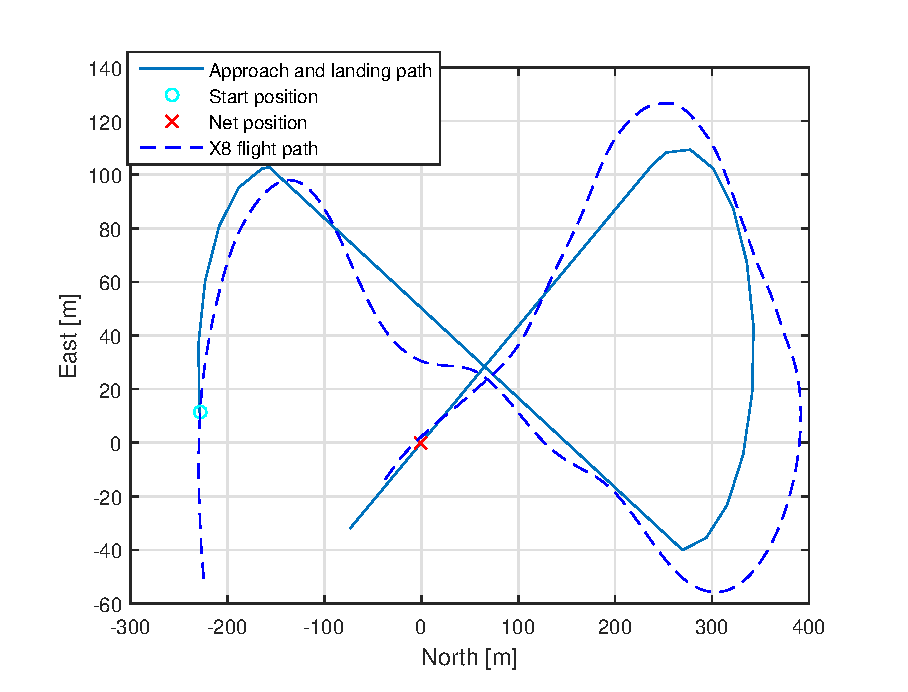
\includegraphics[scale=0.7]{figs/Experiment/NorthEast31mai103029.eps}
		\caption{North-East plot of a landing plan}
		\label{Fig:NorthEast31mai103029}
\end{figure}
\begin{figure}[H]
\centering
		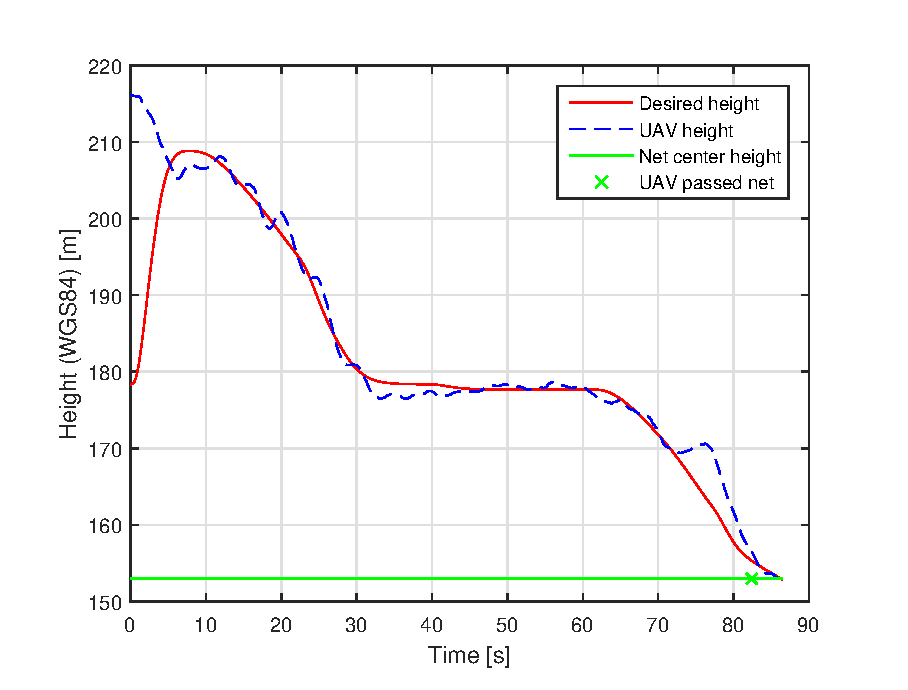
\includegraphics[scale=0.7]{figs/Experiment/Height31mai103029.eps}
		\caption{Height profile of landing plan with $3 \deg$ net impact angle}
		\label{Fig:Height31mai103029}
\end{figure}
\subsubsection{Path with $\gamma_n = 0$}
A new landing plan, where the desired height and \gls{uav} during the landing plan is shown in figure \ref{Fig:Height31mai31mai105034}, was generated with the net impact angle $\gamma_n = 0$. The effect of setting the net impact angle to zero gave a better performance from the longitudinal control system, due to the desired height now converging to the net center height. At the time the \gls{uav} passed the virtual net the hight error with respect the height of the net center was within the height error acceptance.
\begin{figure}[H]
\centering
		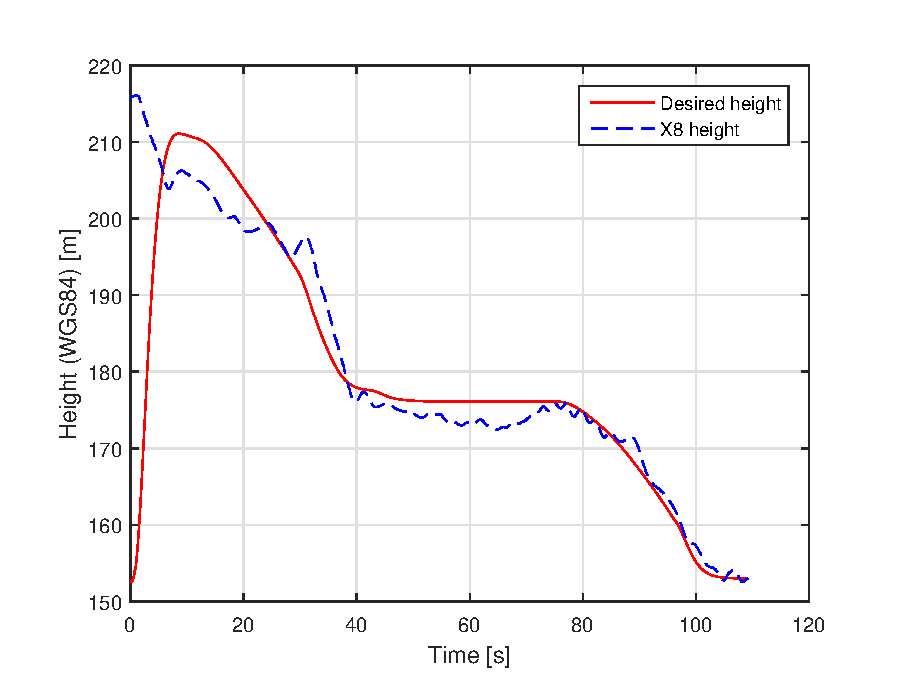
\includegraphics[scale=0.7]{figs/Experiment/Height31mai105034.eps}
		\caption{Height profile of landing plan with $0 \deg$ net impact angle}
		\label{Fig:Height31mai31mai105034}
\end{figure}
\subsubsection{Path with inverted rotation direction in the first circle}
An attempt to reduce the oscilatoric motion of the \gls{uav} during the straight line part of the approach path, a new path was created with inverted rotation direction in the first circle, as shown in figure \ref{Fig:NorthEast31mai125420}. The straight line part of the approach path moved the \gls{uav} to fly in the same direction as the wind, which resulted in less oscillatory motion. However the overshoot in the final circle is still present, which is due to a combination of the \gls{uav} turning up against the wind and the lateral controller not being design to follow a turning manoeuvre.
\begin{figure}[H]
	\centering
	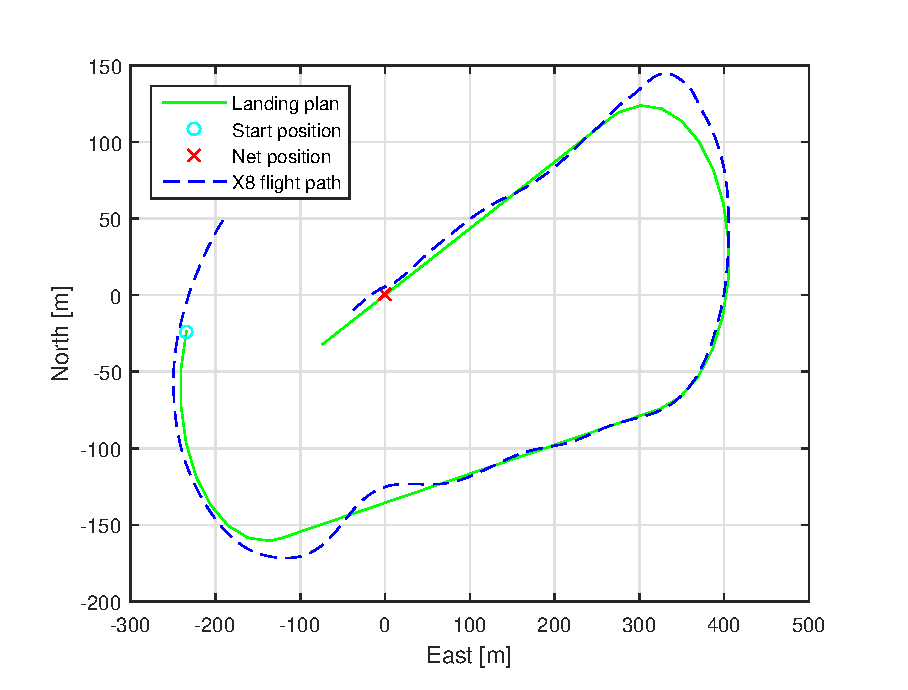
\includegraphics[scale=0.7]{figs/Experiment/NorthEast31mai125420.eps}
	\caption{North-East plot where the straight line segment between the two circles give a path parallel to the wind}
	\label{Fig:NorthEast31mai125420}
\end{figure}
\subsubsection{Path with reduced lookahead distance in lateral controller}
In order to further reduce the oscillatory motion in the lateral plan the lookahead distance in the lateral control system was reduced to make the controller more aggressive towards the wind. The effect of this change is shown in figure \ref{Fig:NorthEast31mai131844}, where the oscillatory motion is almost completely removed. However the overshot at end of the final circle shows that the lateral controller is struggling to handle a turning circle. 
\begin{figure}[H]
\centering
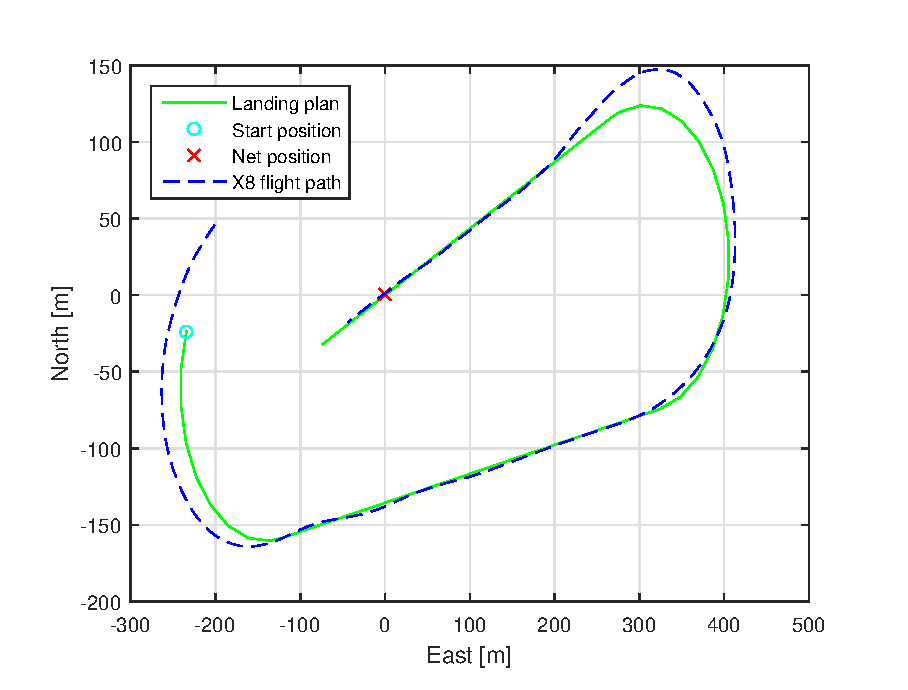
\includegraphics[scale=0.7]{figs/Experiment/NorthEast31mai131844.eps}
\caption{North-East plot where the lookahead distance of the lateral controller was reduced to increase performance when flying against the wind}
\label{Fig:NorthEast31mai131844}
\end{figure}
By reviewing the desired roll ($\phi_d$ ) and the actual roll ($\phi$) of the \gls{uav} at the time of the final turn, shown in figure \ref{Fig:DesiredRoll131844}, it's observed that the lateral control system decrease the desired roll in the middle of the turn. This happens since the lateral control system only sees the next point on the circle, and not the circle as a whole.
\begin{figure}[H]
\centering
\includegraphics[scale=0.7]{figs/Experiment/rollDesired131844.eps}
\caption{The desired roll and actual roll of the \gls{uav}}
\label{Fig:DesiredRoll131844}
\end{figure}
\subsubsection{Summary of day 1}\label{sss:summaryDay1}
The result from the first day was affected with strong wind condition, in which the \gls{uav} struggled to stay on the path and overshooting in the final turning circle. The average heigh and cross track error with respect to desired heigh and path respectfully for 11 landing plan performance, is given in table \ref{tb:Day1HeightCrossTrack}. The average height error vary less then the average cross track error, with a variance of $0.4 m$ against $6.2 m$. However the performance of the \gls{uav} in both height error and cross track error is worse then the results obtain during SIL simulation. This was expected, however the magnitude of the variance in the average cross track error shows that the performance of the lateral control system must increase in order for the autonomous landing system to be considered reliable. 
\begin{table}[H]
\centering
\begin{tabular}{| l | l | l |}
\hline
\textbf{Nr.} 	& \textbf{Average height error [m]} 	& \textbf{Average cross track error [m]}  \\ \hline
$1$				& $1.5$							& $6.1$								\\ \hline
$2$				& $2.6$							& $6.7$								\\ \hline
$3$				& $0.9$							& $5.5$								\\ \hline
$4$				& $0.1$							& $2.8$								\\ \hline
$5$				& $1.7$							& $2.0$								\\ \hline
$6$				& $1.3$							& $6.8$								\\ \hline
$7$				& $1,8$							& $9.1$								\\ \hline
$8$				& $1.2$							& $8.2$								\\ \hline
$9$				& $1.9$							& $5.9$								\\ \hline
$10$			& $1.5$							& $4.4$								\\ \hline
$11$			& $1.5$							& $1.4$								\\ \hline
Average			& $1.5$							& $5.4$								\\ \hline
Variance		& $0.4$							& $6.2$								\\ \hline
\end{tabular}
\caption{Mean height and cross track error from day 1}
\label{tb:Day1HeightCrossTrack}
\end{table}
The variance of the longitudinal control system shows that the control system is reliable in performance, however the average error must decrease to allow increased certainty that the \gls{uav} is able to hit the stationary net. In table \ref{tb:Day1LandingAttempt} the results of whether the \gls{uav} passed through the net or not, is present. Most of the alteration on the path and controllers was aimed towards the lateral control system, which is shown be be increased performance during the later attempts. In the comparison to the simulation results, where the average error was almost zero, the performance has clearly decreased. This behaviour was expected due the simulation model used in the simulation has not been verified. In addition the simulation results was obtain after the two experimental test day, where a different time constant was used in the smoothing filter in the longitudinal control system \citep{Sigurd}. It is expected that this alteration would have increased the behaviour of longitudinal control system, however this has not been verified due to limitation in flight days.
\begin{table}[H]
\centering
\begin{tabular}{| p{0.5cm} | p{1cm} | p{1cm} | p{3.5cm} | p{3cm} | p{1cm} |}
\hline
\textbf{Nr.}	& \textbf{Height error [m]}	& \textbf{Cross track error [m]}& \textbf{Height acceptance}& \textbf{Cross track error acceptance}	& \textbf{Net hit}\\ \hline
$1$				& $2.8$		& $2.1$		& X								& OK									& X					\\ \hline
$2$				& $2.7$		& $-4.5$	& X								& X										& X					\\ \hline
$3$				& $0.9$		& $-1.6$	& OK							& OK									& OK				\\ \hline
$4$				& $0.0$		& $5.4$		& OK							& X										& X					\\ \hline
$5$				& $0.8$		& $5.3$		& OK							& X										& X					\\ \hline
$6$				& $2.1$		& $-1.6$	& X								& OK									& X					\\ \hline
$7$				& $0.7$		& $2.3$		& OK							& OK									& OK				\\ \hline
$8$				& $-1.5$	& $-5.4$	& X								& X										& X					\\ \hline
$9$				& $1.9$		& $0.8$		& X								& OK									& X					\\ \hline
$10$			& $0.3$	& $1.1$		& OK							& OK									& OK				\\ \hline
$11$			& $-1.3$	& $0.2$		& OK							& OK									& OK				\\ \hline
\end{tabular}
\caption{Table containing the result of each landing attempt}
\label{tb:Day1LandingAttempt}
\end{table}
The content of table \ref{tb:Day1LandingAttempt} is shown in figure \ref{Fig:Day1NetPass}, where the net is marked as a whole line and all landing attempts are marked as crosses. The oscillatory motion in the lateral plane by the \gls{uav} is reflected in the placement of the crosses. However the placement of the cross shows the effect of a to high average height error by either passing over the net or in the upper part of the net.
\begin{figure}[H]
\centering
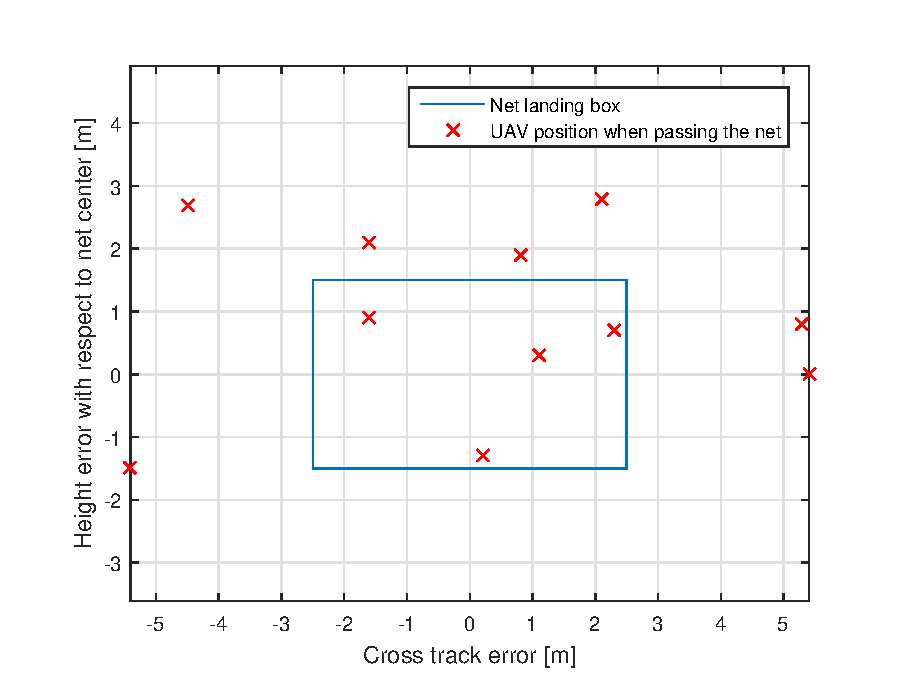
\includegraphics[scale=0.7]{figs/Experiment/day1NetHit.eps}
\caption{Position of UAV relative to the net center at the time of net passing}
\label{Fig:Day1NetPass}
\end{figure}
During the execution of the landing plan it was discovered that in order for the \gls{uav} to stay above the highest tree tops it had to start its decent from an height of $56 m$ above the airfield. Flying bellow this height would result in the pilot losing sight of the \gls{uav}, which is unacceptable in a LOS \gls{uav} operation. This didn't provide a problem during landing attempt with a virtual net which was placed $26 m$ above the airfield, however during a real stationary net landing it would push the limitation of the operation area in which the \gls{uav} can fly. The flight is a Line Of Sight operation, meaning that the pilot must have the \gls{uav} within sight during the entire flight. A $56 m $ decent with a glide slope angle of $6\deg$ would require a glide slope of $500 m$. An estimate of the the available length of which the \gls{uav} can use to perform a autonomous landing in a stationary net is estimated to be $700 m$. This would require the use of the entire runway at Agdenes. An alternative solution is to attempt to land with a greater glide slope angle, or simply start the landing path from West. Landing attempts from the west has yet to tried, the reason being limited time and that would mean that the \gls{uav} would land in the same direction the wind is typically blowing. This would increase the ground speed of the \gls{uav}, which is undesired. However in the case where the wind is calm enough to be considered negligible, a autonomous landing from west would be a valid option.
\subsection{Day 2}
\subsubsection{First path}
The second day had calm wind condition, which is considered as ideal field test conditions for the autonomous landing system. In an attempt to increase the height difference between the start height of the landing path and the net center, a longer glide slope was attempted. The virtual net was place further to the west along the runway, and the length and angle of the glide slope was increase to $280 m$ and $8 \deg$ respectfully. The full path specification for the first path is given in appendix \ref{AP:SpecDay2}.

The path generated with the new parameters is shown in figure \ref{Fig:NorthEast1juni081328}. The lateral path overshoots in both the start and final turning circles. As seen in figure \ref{Fig:Roll1juni081328} the roll motion of the \gls{uav} does not follow the desired roll, which is due to the low level roll controller is tuned for manual flight where rapid changes in the actuators is undesired. In addition the control surface used to control the roll of the \gls{uav} is also used to control the pitch, which results in having to weight the performance in heading against the ability to follow a height reference.
\begin{figure}[H]
\centering
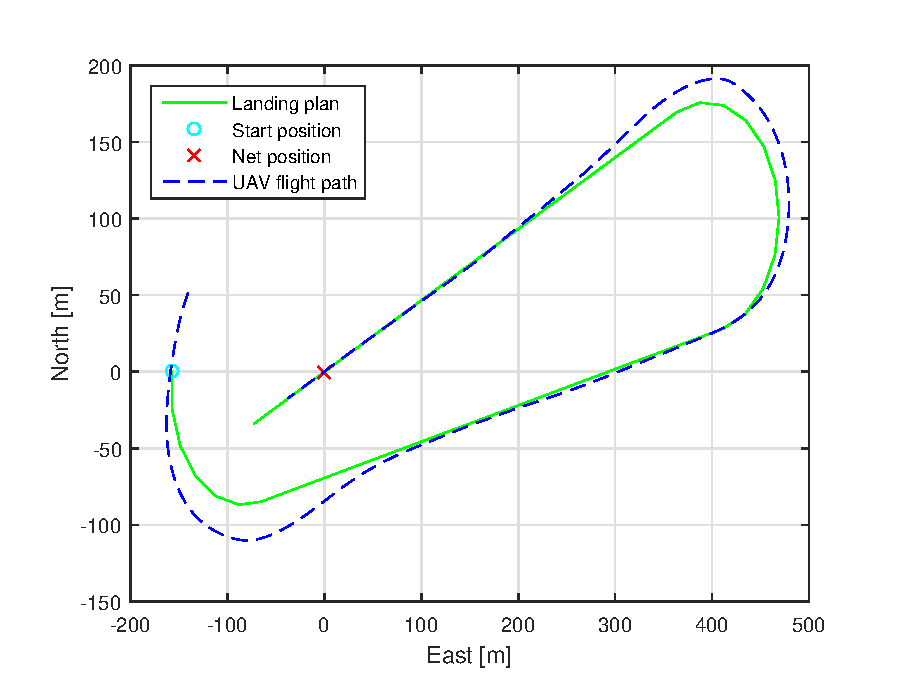
\includegraphics[scale=0.7]{figs/Experiment/NorthEast1juni081328.eps}
\caption{North-East plot}
\label{Fig:NorthEast1juni081328}
\end{figure}
\begin{figure}[H]
\centering
\includegraphics[scale=0.7]{figs/Experiment/Roll1juni081328.eps}
\caption{Roll}
\label{Fig:Roll1juni081328}
\end{figure}
The resulting desired height and \gls{uav} height from the new path, shown in figure \ref{Fig:Height1juni081328}, shows that the \gls{uav} was unable to follow a glide slope with glide slope angle $\gamma_l = 8 \deg$. A major reason for this behaviour is due to the failure of the \gls{uav} pitch to follow the desired pitch, as shown in figure \ref{Fig:Pitch1juni081328}. The pitch appear to to saturated in the low level controller since it does not reach the desired pitch. Better tuning of the low level control system might reduce the bias and lag between actual and desired pitch value, however the reason for the saturation must be further investigated. A restriction in the desired pitch available for the control system, indicate that a new strategy is need in a autonomous landing system where speed assignment during the landing path must be investigated.
\begin{figure}[H]
\centering
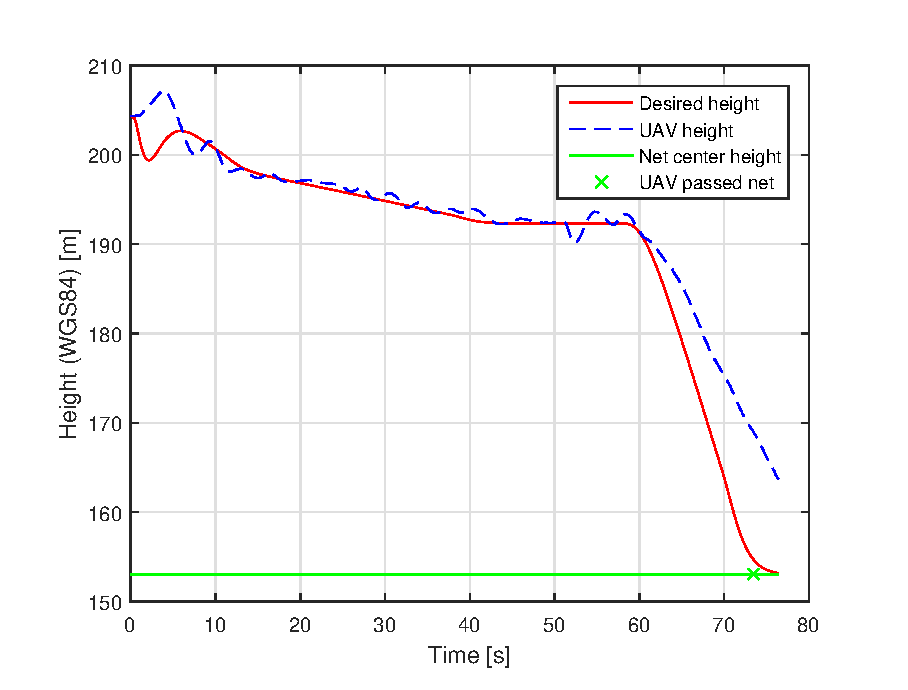
\includegraphics[scale=0.7]{figs/Experiment/Height1juni081328.eps}
\caption{Height}
\label{Fig:Height1juni081328}
\end{figure}
\begin{figure}[H]
\centering
\includegraphics[scale=0.7]{figs/Experiment/Pitch1juni081328.eps}
\caption{Pitch}
\label{Fig:Pitch1juni081328}
\end{figure}
In order to reduce the overshot in the final turning circle the distance between each arc segments each turning circle was reduced. The goal for with this alteration was to get the lateral controller to keep the roll angle in order to increase the turning performance. Figure \ref{Fig:NorthEast1juni083423} shows the the resulting path when the arc segment distance is reduced. The overshot in the final turning circle is reduced, and the cross track error in the final turning circle is shown in figure \ref{Fig:CrossTrackError1juni083423} indicates that the performance of the \gls{uav} increase with short distance between arc segments. A long term solution for reducing overshot in a turning circle would be a dedicated controller for turning manoeuvre. If combined with the current lateral controller which is designed to stay on a straight line between way-point the result will be a controller that is well suited for performing a autonomous landing.
\begin{figure}[H]
\centering
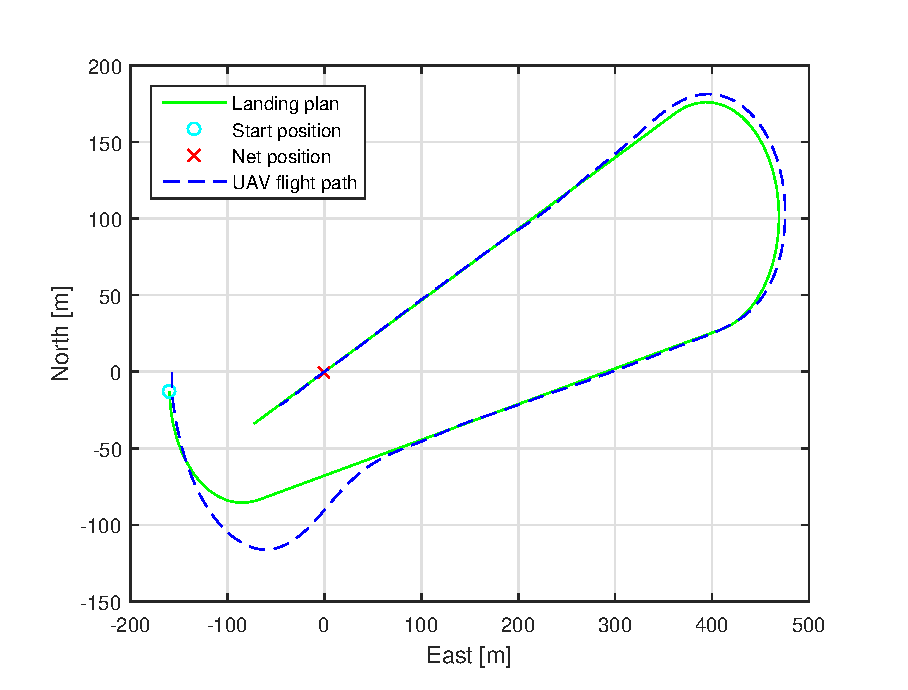
\includegraphics[scale=0.7]{figs/Experiment/NorthEast1juni083423.eps}
\caption{North-East plot where the distance between each arc segments has been reduced from $25 m$ to $10 m$}
\label{Fig:NorthEast1juni083423}
\end{figure}
\begin{figure}
\centering
\includegraphics[scale=0.7]{figs/Experiment/Roll1juni083423.eps}
\caption{Roll and desired roll in the final turning circle}
\label{Fig:RollFinalTurning083423}
\end{figure}
\begin{figure}[H]
\centering
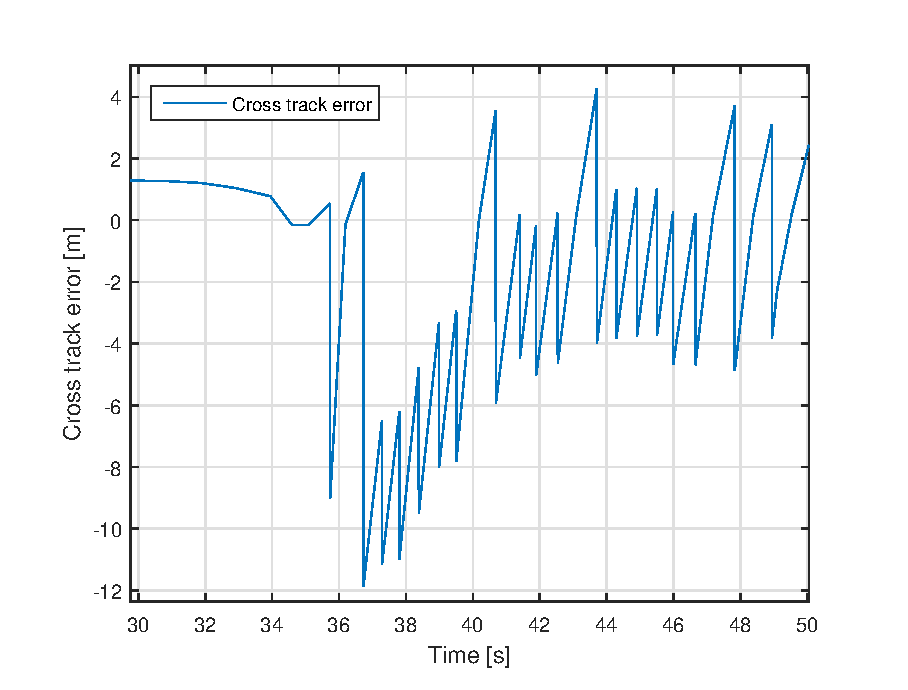
\includegraphics[scale=0.7]{figs/Experiment/CrossTrackError1juni083423.eps}
\caption{Cross track error in the final turning circle}
\label{Fig:CrossTrackError1juni083423}
\end{figure}
\subsubsection{Summary day 2}
The second day had more experimental testing then the first day, where the limits of the height profile and reducing the overshoot in the final turning circle was the main focus. The testing of limits for glide slope angle is reflected in table \ref{Tb:AverageCrossHeightDay2} where the net misses is due to height error. With the current system the limit was found to be $\gamma_l=6\deg$, however better tuning of low level pitch controller and reducing landing speed could increase the limitation on the glide slope angle. The short final approach length resulted in the \gls{uav} to have a short distance of which the net center height could be reached. A longer final approach would result in a higher success rate, however this would require either a longer landing path or shorter glide slope. The final approach could be increased to $120 m$ by moving the net further west over. The risk with a large final approach during a autonomous landing in a real net would be the prolonged time the \gls{uav} flies $3-4 m$ above ground. A loss of high accurate positioning system could then result in a crash.
\begin{table}[H]
\centering
\begin{tabular}{| l | l | l |}
\hline
\textbf{Nr.} 	& \textbf{Average height error [m]} 	& \textbf{Average cross track error [m]}  \\ \hline
$1$				& $2.2$							& $3.8$										\\ \hline
$2$				& $1.2$							& $3.4$										\\ \hline
$3$				& $0.9$							& $-1.8$									\\ \hline
$4$				& $2.5$							& $-0.2$									\\ \hline
$5$				& $3.0$							& $0.3$										\\ \hline
$6$				& $1.6$							& $0.2$										\\ \hline
$7$				& $1,9$							& $-2.3$									\\ \hline
$8$				& $1.9$							& $-0.1$									\\ \hline
Average			& $1.9$							& $0.5$										\\ \hline
Variance		& $0.5$							& $4.7$										\\ \hline
\end{tabular}
\caption{Average height and cross track error from day 2}
\label{Tb:AverageCrossHeightDay2}
\end{table}

\begin{table}[H]
\centering
\begin{tabular}{| p{0.5cm} | p{1cm} | p{1cm} | p{3.5cm} | p{3cm} | p{1cm} |}
\hline
\textbf{Nr.}	& \textbf{Height error [m]}	& \textbf{Cross track error [m]}& \textbf{Height acceptance}& \textbf{Cross track error acceptance}	& \textbf{Net hit}\\ \hline
$1$				& $14.4$		& $0.1$		& X								& OK									& X					\\ \hline
$2$				& $1.3$		& $0.6$	& OK								& OK										& OK					\\ \hline
$3$				& $1.1$		& $-0.2$	& OK							& OK									& OK				\\ \hline
$4$				& $1.4$		& $0.1$		& OK							& OK										& OK					\\ \hline
$5$				& $1.1$		& $0.1$		& OK							& OK										& OK					\\ \hline
$6$				& $2.0$		& $-0.2$	& X								& OK									& X					\\ \hline
$7$				& $2.3$		& $0.2$		& X								& OK									& X				\\ \hline
$8$				& $7.0$	& $0.3$	& X										& OK										& X					\\ \hline
\end{tabular}
\caption{Table containing the result of each landing attempt}
\label{tb:Day2LandingAttempt}
\end{table}
\begin{figure}[H]
\centering
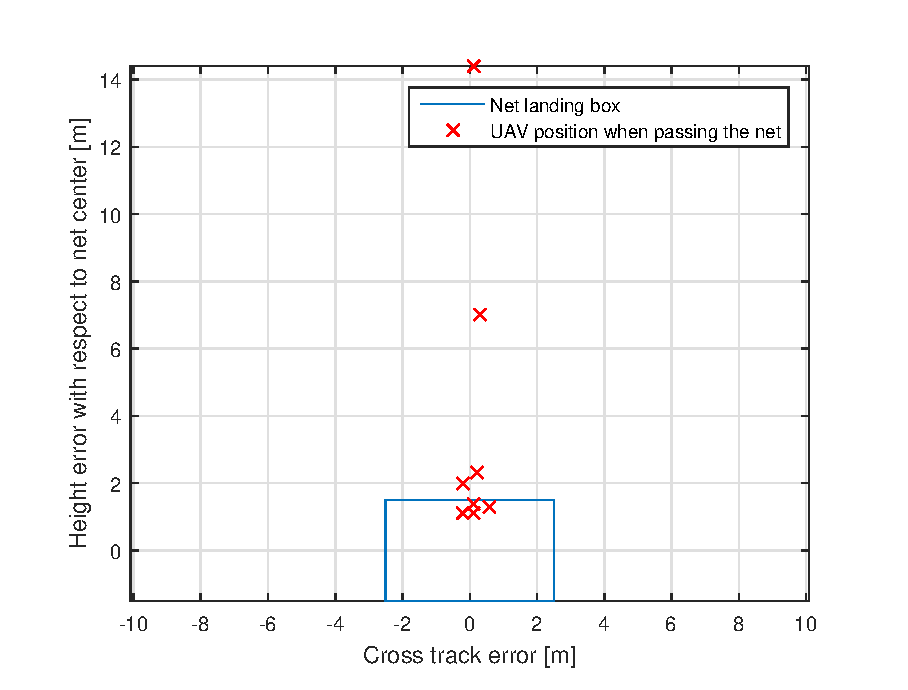
\includegraphics[scale=0.7]{figs/Experiment/day2NetHit.eps}
\caption{Position of the \gls{uav} relative to the net center at the time of net passing}
\label{Fig:Day2NetPass}
\end{figure}
The performance of the lateral controller increase during calm wind condition, however the performance of the longitudinal controller is the same as during windy conditions. Table \ref{Tb:AverageCrossHeightDay2} list up the average height error and cross track error relative to the desired height and path. 
\section{Navigation}\label{ss:EXNavigation}
The testing of the navigation system is restricted to the X8, however the same navigation system was used in a multicoper \gls{uav} both days.
\subsection{RTK-GNSS performance}
The performance of the \gls{rtk-gnss} system during the first day of executing landing plans is summaries in table \ref{TB:RTKFirstDayRTK}, which shows that \gls{rtk-gnss} kept a stable FIX during the landing plan experiment. The same result was achieved during the second day during the execution of the landing plans, however the \gls{rtk-gps} experienced problem later the second day, due to lost contact with the base station. The expected reason is that pore satellite geometry made effective use of \gls{rtk-gps} difficult.
\begin{table}[H]
\centering
\begin{tabular}{| l | l | l | l |}
\hline
\textbf{Nr.}	& \textbf{FIX \%}	& \textbf{FLOAT \%}	& \textbf{NONE \%}	\\ \hline
$1$				& $99.5 $	& $0.5$	& $0.0$									\\ \hline
$2$				& $99.5 $	& $0.5$	& $0.0$									\\ \hline
$3$				& $99.8 $	& $0.0$	& $0.0$									\\ \hline
$4$				& $100$		& $0.0$	& $0.0$									\\ \hline
$5$				& $100$		& $0.0$	& $0.0$									\\ \hline
$6$				& $100$		& $0.0$	& $0.0$									\\ \hline
$7$				& $99.9$	& $0.1$	& $0.0$									\\ \hline
$8$				& $99.7 $ 	& $0.3$	& $0.0$									\\ \hline
$9$				& $99.3$	& $0.7$	& $0.0$									\\ \hline
$10$			& $100$		& $0.0$	& $0.0$									\\ \hline
$11$			& $100$		& $0.0$	& $0.0$									\\ \hline
\end{tabular}
\caption{Performance of the RKT-GNSS system the first day during the executing of the landing plans}
\label{TB:RTKFirstDayRTK}
\end{table}
\subsection{Short loss compensator}
The short loss compensator was designed to prolong the availability of the \gls{rtk-gps}, such that a flight plan does not get interrupted due to a temporary problem with the \gls{rtk-gnss}. During a flight the second day the gls{rtk-gps} experienced a short drop out, as seen in figure \ref{Fig:NavSource}. Even though the \gls{rtk-gps} position solution is unavailable the navigation system is still able to supply high accurate position solution due to the short \gls{rtk-gnss} compensator as seen in figure \ref{Fig:ShortLoss}. The duration of the short \gls{rtk-gps} could be expanded, and currently the time limitation of the compensator where the position solution start to diverge is unknown.
\begin{figure}[H]
\centering
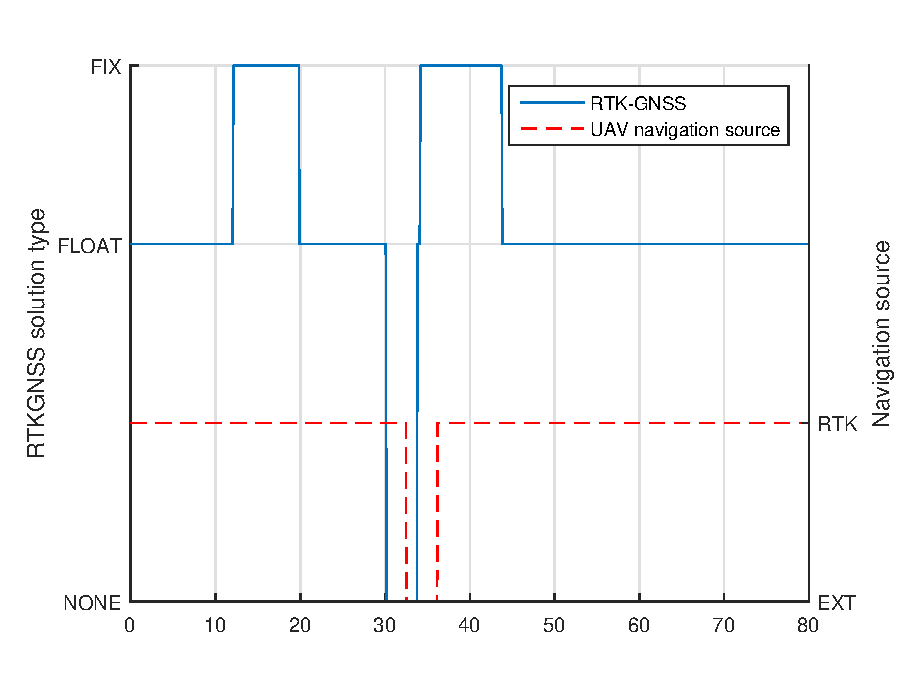
\includegraphics[scale=0.7]{figs/Experiment/navSource.eps}
\caption{State of RTK-GNSS system and \gls{uav} navigation source.}
\label{Fig:NavSource}
\end{figure}
\begin{figure}[H]
\centering
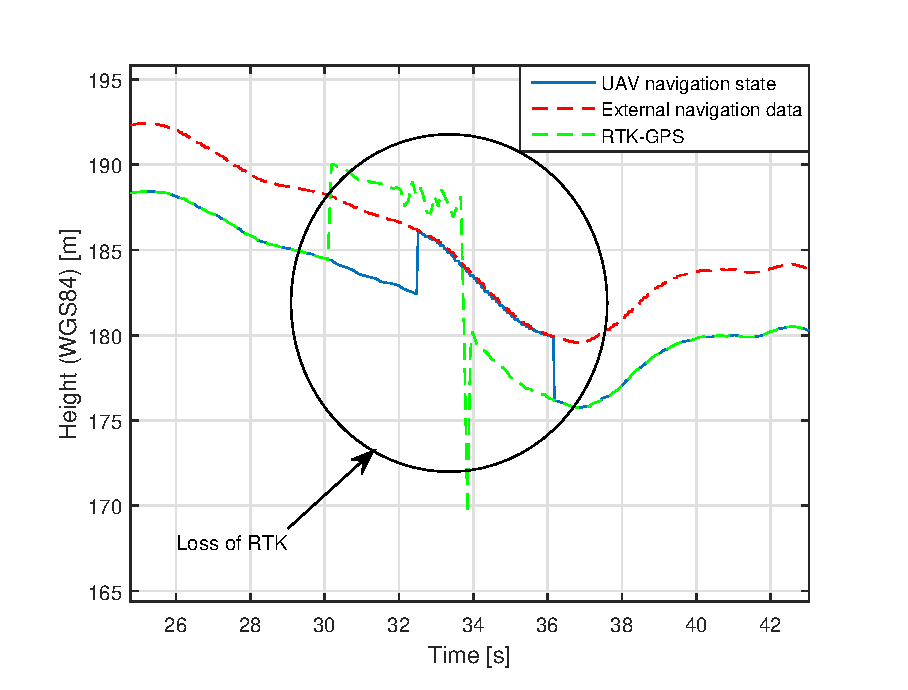
\includegraphics[scale=0.7]{figs/Experiment/shortrtkloss1juni114124.eps}
\caption{Loss of \gls{rtk-gps} triggers the short loss compensator such that the \gls{uav} keeps the \gls{rtk-gps} position solution longer}
\label{Fig:ShortLoss}
\end{figure}
\subsection{Summary of navigation system performance}
\section{Summary}
This chapter showed the performance of a X8 fixed wing \gls{uav} performing a autonomous landing in a virtual net. The performance of the navigation system is acceptable for a autonomous system by supplying a stable highly accurate position solution, with redundancy for short \gls{rtk-gps} loss periods. The landing plan still require further testing to develop path parameters that  will result in a successful net landing. The path parameters are depending on the ability for the control system to follow the desired path, which might prove demanding in the longitudinal plane for large change in high over a short distance.